\chapter{Określanie lokalizacji}
\label{cha:lokalizacja}
\section{Lokalizacja użytkownika}
Lokalizację użytkownika w systemie określa się na podstawie odległości od punktów, których współrzędne w przestrzeni trójwymiarowej są znane. Są to głównie routery i Beacony, jednak może się zdarzyć, że takim punktem staje się również inny użytkownik. Współrzędne użytkownika można obliczyć, dokonując pomiarów wskaźnika mocy \textit{RSSI}, podając siłę sygnałów odebranych przez otaczające go urządzenia i obliczając na ich podstawie dystans \cite{RSC}.
\section{Trilateracja}
Powszechnie wykorzystywanym sposobem obliczenia lokalizacji użytkownika na podstawie dystansu do znanych punktów, jest trilateracja \cite{MS}. Metoda ta polega na przedstawieniu dystansu dzielącego punkt od nadajników w postaci okręgi (lub sfery w przypadku, gdy określamy lokalizację w trzech wymiarach). Następnie, należy wyznaczyć współrzędne punktu przecięcia okręgów \cite{MS}. Wyznaczony punkt jest lokalizacją odbiornika, dla którego dokonywaliśmy obliczenia.
\begin{figure}[H]			
	\centering
	\caption{Wizualizacja modelu trilateracji}
	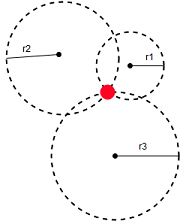
\includegraphics{trilateracja}
\end{figure}
Współrzędną punktu można obliczyć na podstawie wzoru:
\begin{equation}
\left\{
\begin{array}{l}
(x_p-x_1)^2 + (y_p - y_1)^2 = r_1^2\\
(x_p-x_2)^2 + (y_p - y_2)^2 = r_2^2\\
(x_p-x_3)^2 + (y_p - y_3)^2 = r_3^2
\end{array}
\right.
\end{equation}
gdzie:
\begin{itemize}
	\item $x_p$, $y_p$ to współrzędne obliczanego odbiornika
	\item $x_1$, $y_1$, $x_2$, $y_2$, $x_3$, $y_3$ to współrzędne znanych punktów
	\item $r_1$, $r_2$, $r_3$ to odległości między punktem obliczanym, a punktami o znanych współrzędnych
\end{itemize}
Ta metoda lokalizowania użytkownika w przestrzeni ma jedną, bardzo ważną wadę, która wyklucza jej wykorzystanie w tworzonym systemie - nie potrafi się dostosować do błędów pomiarowych, których w przypadku określania lokalizacji przy użyciu sygnałów radiowych, jest dużo. Aby wyznaczone lokalizacje użytkowników w sposób zbliżony odwzorowywały rzeczywiste położenie, algorytm obliczający musiał być bardziej odporny na błędy pomiarowe \cite{MT}.
\section{Lokalizacja jako funkcja probabilistyczna Gaussa}
Z racji tego, iż mierzony sygnał, odbierany przez odbiornik, ulega zniekształceniom i odbiciom, określenie dystansu między transmiterem, a odbiorcą w sposób liniowy jest niezgodne z fizycznymi zachowaniami sygnału. Siła sygnału oraz straty wywołane przez zniekształcenia i odbicia, określone są w jednostce dB. Wynika z tego, że najlepszym przybliżeniem zmian siły sygnału może być funkcja Gaussa \cite{GMBF}. Zamiast określać konkretne położenie użytkownika, w pracy zastosowane będzie podejście, które pozwoli na przedstawienie jego lokalizacji jako prawdopodobieństwo położenia.\\
\subsection{Funkcja probabilistyczna Gaussa}
Funkcja probabilistyczna Gaussa jest to krzywa w kształcie dzwonu, symetryczna względem średniej $\mu$ oraz uzyskująca wartość maksymalną w punkcie $\frac{1}{\sqrt{2\pi}\sigma}$.
Określa się ją za pomocą wzoru:
\begin{equation}
F(x) = \frac{1}{\sigma\sqrt{2\pi}}e^{\left(\frac{-(x-\mu)^2}{2\sigma^2}\right)}
\end{equation}
Zmienne $\mu$ będąca średnią, oraz $\sigma$ będąca odchyleniem standardowym, w pełni opisują tą funkcję \cite{MIR}.
\begin{figure}[H]			
	\centering
	\caption{Wykres funkcji Gaussa dla różnych wartości parametrów}
	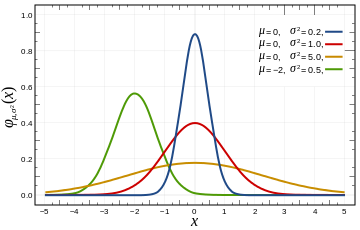
\includegraphics{funkcja_Gaussa}
\end{figure}
Funkcja Gaussa jest szeroko wykorzystywana w statystyce. W elektronice, korzysta się z niej podczas charakteryzowania pomiarów sensorów czy siły sygnałów radiowych.
\subsection{Model routerów jako funkcja Gaussa}
Jeżeli określimy lokalizację odbiornika względem transmitera jako funkcję prawdopodobieństwa Gaussa:
\begin{equation}
F(x) = \frac{1}{\sigma\sqrt{2\pi}}e^{\left(\frac{-(d_o-d)^2}{2\sigma^2}\right)}
\end{equation}
to wartość funkcji określa, jakie jest prawdopodobieństwo, że odbiornik znajduje się w odległości $d_o$ od transmitera. Największe prawdopodobieństwo przypisywane jest dystansowi, który obliczyliśmy z siły sygnału, dlatego to właśnie ta wartość podstawiana jest pod zmienną $d$ \cite{JK}.\\
Jeżeli transmiter opisze się jako funkcję prawdopodobieństwa Gaussa \cite{YX}, wyznaczoną na podstawie odebranej siły sygnału, zwizualizowany model transmitera w przestrzeni dwuwymiarowej przypomina pierścień, którego gęstość maleje wraz z oddalaniem się od obliczonej z mocy sygnału odległości.
\begin{figure}[H]			
	\centering
	\caption{Wizualizacja modelu routera opisanego funkcją Gaussa. Jasność punktów oznacza wielkość prawdopodobieństwa $F(x)$. Na czerwono zaznaczono odległość obliczoną na podstawie siły sygnału transmitera $d$, a zielony prostokąt oznacza lokalizację transmitera. Wartość d wyznaczana jest za pomocą wzoru $d = \sqrt{d_x^2 + d_y^2}$.}
	
\includegraphics[width=0.75\textwidth]{router_Gaussa_wizualizacja}
\end{figure}
\subsection{Lokalizacja użytkownika opisana funkcją Gaussa}
Wyżej opisane podejście, poza realniejszym oddaniem natury rozchodzenia się sygnału w środowisku \cite{TDECHN}, ma również dodatkową zaletę - w łatwy sposób można wyliczyć prawdopodobieństwo położenia odbiornika wtedy, gdy w modelu znajduje się więcej transmiterów.\\
Jednym ze sposobów określenia położenia użytkownika jest zsumowanie prawdopodobieństw obliczonych w każdym punkcie w przestrzeni z funkcji Gaussa przypisanych do transmiterów. Prawdopodobieństwo dla puntu $(X,Y)$ może być określone na podstawie wzoru:
\begin{equation}
F(X,Y) = \sum_{r=1}^{R} \frac{1}{\sigma_r\sqrt{2\pi}}e^{\left(\frac{-(D(X,Y,r)-d_r)^2}{2\sigma_r^2}\right)}
\end{equation}
w którym kolejne symbol oznaczają:
\begin{itemize}
	\item $R$ - zbiór transmiterów. Z racji tego, iż funkcja Gaussa przyjmuje wartości większe od zera dla całego zakresu $(-\infty,\infty)$, wartość prawdopodobieństwa jest liczona dla każdego transmitera, niezależnie od tego, jak daleko znajduje się on od punktu $(X,Y)$
	\item $D(X,Y,r)$ - euklidesowa odległość punktu $(X,Y)$ od transmitera $r$
	\item $d_r$ - odległość obliczona na podstawie siły sygnału transmitera $r$
	\item $\sigma_r$ - odchylenie standardowe - wartość wyznaczana na podstawie odległości transmiterów od odbiornika. Dodatkowo, z racji tego, iż sygnał Wi-Fi jest bardziej odporny na nagłe zaniki wynikające ze wzrostu odległości, niż sygnał Bluetooth \cite{BLUE}, wartość odchylenia skalowana jest w zależności od tego, jaki typ sygnału wysyła konkretny transmiter.\\
	Wartość $sigma_r$ można obliczyć za pomocą wzoru:
	\begin{equation}
		\sigma_r = \frac{D_m * w_r}{30}
	\end{equation}
	gdzie $D_m$ to długość najdłuższego boku modelu, tworzonego przez sygnały ze wszystkich transmiterów, a $w_r$ to waga sygnału, który wysyła transmiter $r$
\end{itemize}
Po ustaleniu wartości dla wszystkich punktów w przestrzeni, jako lokalizacja odbiornika przyjęty zostaje taki punkt $(X_o,Y_o)$, którego suma prawdopodobieństw jest najwyższa.
\begin{figure}[H]			
	\centering
	\caption{Model lokalizacji odbiornika wykonany w programie MatLab. Punkt o największym prawdopodobieństwie oznaczony jest za pomocą czarnej strzałki.}
	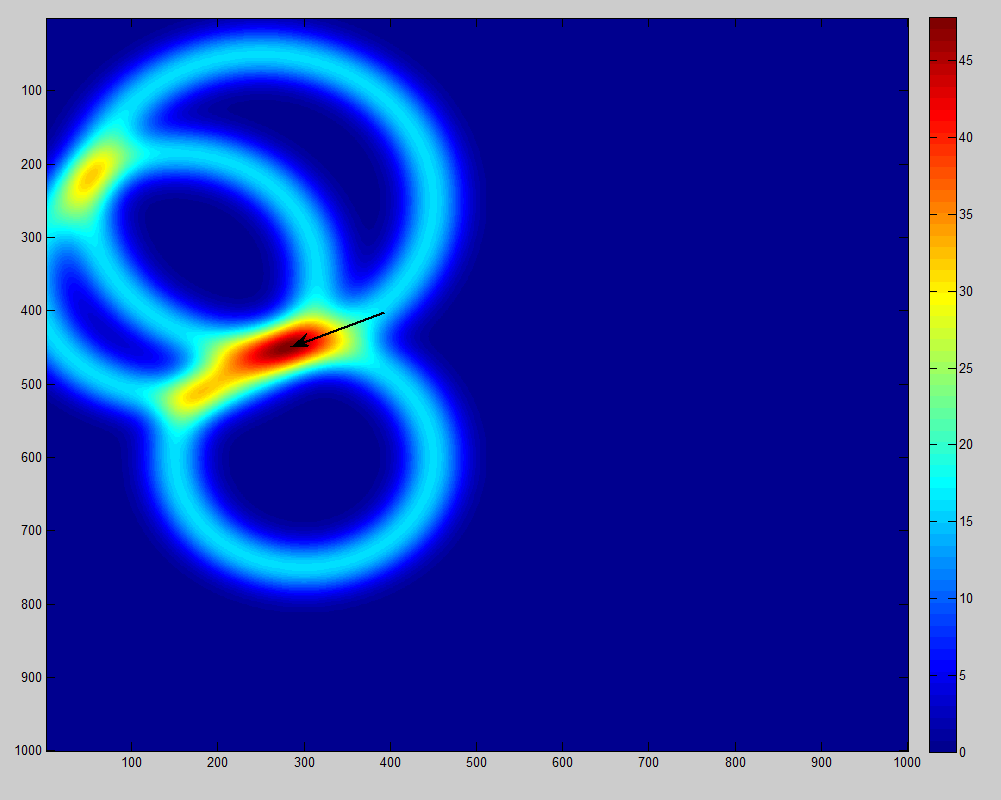
\includegraphics[width=0.75\textwidth]{guasianRouter}
\end{figure}
Zaprezentowany sposób wyznaczania lokalizacji dotyczył obliczeń w przestrzeni dwuwymiarowej. Przejście na przestrzeń trójwymiarową nie stanowi problemu - jedynymi zmianami, jakie należy wprowadzić, są:
\begin{itemize}
	\item wykonywanie obliczeń dla punktów $(X,Y,Z)$
	\item zmiana sposobu obliczania odległości euklidesowej między odbiornikiem, a transmiterem - należy wyznaczać odległość w przestrzeni trójwymiarowej.
\end{itemize}
